% A plane tree with 9 vertices and its contour walk, a Dyck path of length 16: walking around the tree, each edge is crossed once down (up-step) and once up (down-step). Generated by a short script.
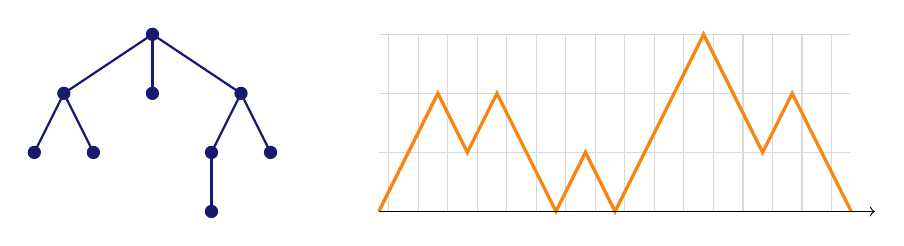
\begin{tikzpicture}
\draw[MidnightBlue,thick] (0.750,-0.750)--(0.375,-1.500);
\draw[MidnightBlue,thick] (0.750,-0.750)--(1.125,-1.500);
\draw[MidnightBlue,thick] (2.625,-1.500)--(2.625,-2.250);
\draw[MidnightBlue,thick] (3.000,-0.750)--(2.625,-1.500);
\draw[MidnightBlue,thick] (3.000,-0.750)--(3.375,-1.500);
\draw[MidnightBlue,thick] (1.875,0.000)--(0.750,-0.750);
\draw[MidnightBlue,thick] (1.875,0.000)--(1.875,-0.750);
\draw[MidnightBlue,thick] (1.875,0.000)--(3.000,-0.750);
\fill[MidnightBlue] (0.375,-1.500) circle (2.4pt);
\fill[MidnightBlue] (1.125,-1.500) circle (2.4pt);
\fill[MidnightBlue] (0.750,-0.750) circle (2.4pt);
\fill[MidnightBlue] (1.875,-0.750) circle (2.4pt);
\fill[MidnightBlue] (2.625,-2.250) circle (2.4pt);
\fill[MidnightBlue] (2.625,-1.500) circle (2.4pt);
\fill[MidnightBlue] (3.375,-1.500) circle (2.4pt);
\fill[MidnightBlue] (3.000,-0.750) circle (2.4pt);
\fill[MidnightBlue] (1.875,0.000) circle (2.4pt);
\draw[black!15] (4.75,-2.250) grid[xstep=0.375,ystep=0.75] (10.750,0);
\draw[BurntOrange,very thick] (4.750,-2.250)--(5.125,-1.500)--(5.500,-0.750)--(5.875,-1.500)--(6.250,-0.750)--(6.625,-1.500)--(7.000,-2.250)--(7.375,-1.500)--(7.750,-2.250)--(8.125,-1.500)--(8.500,-0.750)--(8.875,0.000)--(9.250,-0.750)--(9.625,-1.500)--(10.000,-0.750)--(10.375,-1.500)--(10.750,-2.250);
\draw[->] (4.75,-2.250)--(11.050,-2.250);
\end{tikzpicture}
